\documentclass{article}
\usepackage[english]{babel}
\usepackage[utf8]{inputenc}
\usepackage{fancyhdr}
\usepackage[square]{natbib}
\usepackage{multibib}
\newcites{main}{Primary References}
\bibliographystyle{apalike}
\bibliographystylemain{apalike}
\newcites{code}{Code References}
\bibliographystylecode{apalike}
\newcites{soft}{Software References}
\bibliographystylesoft{apalike}
\usepackage{graphicx}
\graphicspath{ {./Images/} }
\usepackage{wrapfig}
\setlength{\abovecaptionskip}{7pt plus 3pt minus 2pt}
\usepackage{geometry}
\geometry{a4paper,left=30mm,top=30mm}
\usepackage{float}
\usepackage{hyperref}

%Titlepage
\thispagestyle{fancy}
\fancyhf{}
\setlength{\headheight}{22.54448pt}
\rhead{University of Sussex - Informatics\\
Computer Science with Artificial Intelligence}
\lhead{Jacob Brown}
\rfoot{
Submission Year - 2022\\
Candidate Number - 198732\\
Project Supervisor - Simon Bowes\\
\url{https://github.com/jacobgeorge26/lizardbot}
}

\begin{document}
\paragraph*{
\\
}
\part*{
\begin{center}
{ \Huge ``Lizardbot"}
\\[1\baselineskip]
{\Large A reptile-inspired model of robots optimised to navigate rough terrain}
\\[1\baselineskip]
\end{center}
}
\section*{Abstract}
Lizardbot aims to provide a solution derived from natural processes for robots traversing irregular environments. Unity software was used to create a model of these robots with realistic physics interaction. The design combined a serpentine motion of the body, the use of a tail for stabilisation, and a lizardlike gait. An AI sought an optimal design by evolving the robots, mutating the physical structure and movement algorithms in tandem. Lizardbot was able to find an optimisation on the less extreme terrains: a single spherical body module with emergent rolling behaviour. Lizardbot demonstrated that a nature-inspired algorithm will not necessarily produce a naturalistic result.

\vspace*{\fill}
\newpage
\pagestyle{fancy}
\fancyhf{}
\rhead{PAGE \thepage}
\lhead{LIZARDBOT}

\newpage
\section*{Statement of Originality}
This  report  is  submitted  as  part  requirement  for  the  degree  of  Computer  Science  and  Artificial 
Intelligence at the University of Sussex. It is the product of my own labour except where indicated in 
the text. The report may be freely copied and distributed provided the source is acknowledged. I hereby 
give permission for a copy of this report to be loaned out to students in future years.

\section*{Professional and Ethical Considerations}
\label{sec:Ethics}
This project will be an isolated model without any user testing, personal data, vulnerable people, protected characteristics, or medical data. While it does focus on reptiles there will not be any experimentation on any animals. Referenced studies will have faced their own ethical review and will largely use videos of the animal being studied. All testing will be conducted by comparing various inputs to the code and analysing the results.\\
With these considerations, this project has been classed as low-risk.\\

This project will abide by the \textbf{BSC Code of Conduct}\footnote{\url{https://www.bcs.org/media/2211/bcs-code-of-conduct.pdf}} regarding:
\begin{itemize}
 \item Public Interest;
 \item Professional Competence and Integrity;
 \item Duty to Relevant Authority;
 \item Duty to the Profession.
 \end{itemize}

%https://tex.stackexchange.com/questions/405195/change-the-length-of-footnote-line
\makeatletter
\renewcommand\footnoterule{\kern-3\p@\hrule\@width\ifodd\value{page}6in\else6in\fi\kern2.6\p@}
\makeatother 

\newpage
\pagestyle{fancy}
\fancyhf{}
\rhead{PAGE \thepage}
\lhead{LIZARDBOT - \leftmark}
\tableofcontents

%Report
\newpage
\section{Introduction}
\label{sec:Introduction}
Nature can often inspire elegant and efficient solutions to non-natural problems. The tunnel-building behaviours of ants can be used to generate algorithms to manage traffic flow in a city for example. This can be much more efficient than deploying a group of developers to design an elaborate network to structure how the population navigates the city. Instead, the nests of ants could be studied and their tunnel-building algorithm applied to the problem \citepmain{antCars}. \\

On a climbing trip to the Isle of Portland I took a break from repeatedly falling off the cliff to watch a lizard. It was attempting to jump from the path onto a nearby rock. Every time it failed it paused, then tried again with its tail in a completely different position. It was naturally using its tail to counterbalance its body as it jumped, and learning from previous attempts. The addition of a tail to a robot can produce an efficient jumping robot with the application of relatively simple maths. A prime example of this is shown in the \textit{‘UC Berkeley Leaping Lizard \& Robot}’ video \citepmain{agamaVideo}. This behaviour can be observed elsewhere in nature; when a praying mantis jumps it swings its body and abdomen to ensure it hits its target \citepmain{prayingMantis},  or when cats twist their bodies to reorient themselves to land on their feet \citepmain{catsLanding}.\\

In this project, the characteristics of various reptiles will be applied to a model of a robot - “Lizardbot” - to optimise the physical design and algorithm it uses to navigate rough terrain. For robots used in applications such as bomb disposal or interplanetary exploration, the environments that they face can be highly unpredictable. The margin for error is often low to nonexistent, as there can be little physical access to the robot to fix any issues. These robots require a design and an algorithm optimised to enable them to traverse any landscape they are presented with. The stabilising tail of a lizard, alongside other reptilian characteristics, could provide a nature-inspired solution for a robot targeting rough terrain.\\

The robots will be modelled due to the resources required to build a physical robot. Even if it were possible to conduct physical testing, for applications such as extraterrestial robots the testing would still depend on simulations.\\
To construct a virtual model of the robot, the popular gaming engine Unity \citepsoft{unity} will be used. The Unity engine has built-in physics, collision, and terrain features that bring complex interactions within scope.


\newpage
\section{Project Aims}
\label{sec:Project Aims}
This project will focus on determining how various reptilian characteristics influence the success of the model as it navigates a terrain. The objective is to explore the ‘ideal’ design of a robot, and the relationship between this body and its navigation of a randomly generated terrain. The basic performance metric will be how far it successfully moves across the terrain (in a straight line from the origin) before it gets stuck. This final state may be bouncing back and forth between two points or hitting a section of the terrain that it cannot progress past; the algorithm to determine if the robot is trapped will consider both of these possibilities. \\
Within this bigger picture goal there will be several smaller experiments into how various features / approaches influence the outcome. \\

Lizardbot will be constructed as a model of a robot due to the resources required to build a physical robot. Having prior experience with Unity \citepsoft{unity} I was confident that its physics system would provide realistic behaviour. Given this, the free access, vast range of functionality and excellent documentation, the decision was made to proceed using Unity. \\

\subsection{Primary Objectives}
\label{sec:Primary Objectives}
\subsubsection{Robot Design}
\label{sec:Robot Design}
The body of the robot will emulate that of a snake such that it will be constructed of a series of independent modules / sections located linearly behind the head. This design \textit{"provides the ability of traversing in irregular environments, something that surpasses the mobility of the conventional wheeled, tracked and legged types of robots"} \citepmain[p. 536]{modularDesign}.\\
Legs will be added at random positions perpendicular to the body and rotate $360^\circ$ to push the body forward. A tail, added behind the body, will rotate to counterbalance the motion of the body. Every joint will have a constraint defining how far it is capable of rotating around each axis. \\

There will be an option to generate robots with random parameters, from the number of body modules and legs, to the force with which they drive. Additionally, a boolean option will determine if the robot is constructed 'uniformly' - i.e. asserting whether it must be symmetrical with all legs / body modules of equal size and mass to each other. The ideal parameters for both the physical design and movement of a robot will be explored.\\

To simplify the model of the robot it will be constructed of basic shapes. The body will be a string of spheres, whilst the legs and tail will be spheroids. The decision against cubes/cuboids is to prevent the shapes from ‘catching’ on anything, as this could interfere with the results. Of course, with a physical robot there will be this interaction to contend with; for the purpose of the model it has been assumed that each surface is uniform and can be smoothed for simplicity. \\

\begin{figure}[H]
\centering
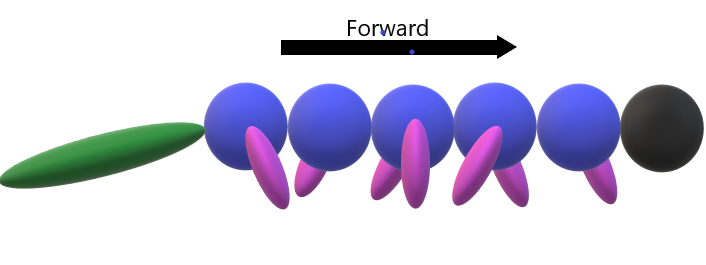
\includegraphics[scale=0.5]{robotDesign}
\caption{An example of a randomly generated robot (viewed from the side).}
\end{figure}

\newpage
\subsubsection{Body Movement}
\label{sec:Body Movement}
\begin{wrapfigure}[17]{r}{0.3\textwidth}
    \centering
    \vspace*{-5mm}
    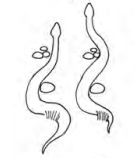
\includegraphics[width=0.3\textwidth]{serpentine}
    \vspace*{-7mm}
\caption{Diagram of a snake using a serpentine method of locomotion \citep{reptileLocomotion}.}
    \label{fig:snakeMethods}
\end{wrapfigure}
The fundamental movement pattern of the body sections will mimic the serpentine motion of a snake, as shown in \autoref{fig:snakeMethods}.

To achieve this, each module will have the ability to drive forward and/or rotate and will have its own set of parameters (e.g. speed). To improve the fluidity of the motion a central pattern generator (CPG) approach will be taken. A CPG \textit{"can produce rhythmic motor patterns ... in the absence of sensory or descending inputs that carry specific timing information"} \citepmain[p. 986]{cpgDefinition}. It is worth noting that the body will not implement a true CPG: the algorithm will utilise a similar approach that avoids any sensory understanding of its worldspace or timing.\\

There will be an option to maintain serpentine motion by alternating the direction of rotation between the rotating sections, and evenly spacing these sections across the body (see \autoref{fig:serpentineDiagram}). The algorithm will not be constrained to this serpentine motion so may move away from this behaviour as it mutates. Nonetheless, due to the embodiment of the robot it is expected that the motion will remain snakelike.\\
\begin{figure}[H]
\centering
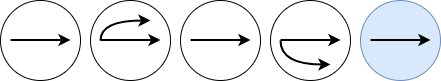
\includegraphics[scale=0.6]{serpentineDiagram}
\caption{The driving \& rotation values used to maintain a serpentine motion.}
\label{fig:serpentineDiagram}
\end{figure}

The decision to have the body oscillate (as opposed to remaining static whilst the legs provide the entirety of the motion) is supported by Jeongryul Kim \citepmain{bodyOscillation}. Due to a lack of degrees of freedom in legged robots a robot may struggle to maintain its posture and direction of movement. \textit{"A possible solution to such lack of DOFs caused by underactuation may be additional motions of the body"} \citepmain[p. 130]{bodyOscillation}.
It is important to note that the referenced study was analysing bipedal robots when this conclusion was drawn. To test the assumption that moving the body with the legs improves performance, another experiment will be conducted to explore the impact of the body remaining static. \\
An alternative solution could be to add additional joints for the legs to increase the DOFs. For Lizardbot, a form that mimicked the structure of a lizard was prioritised whilst considering the positioning of leg joints. The offer of freedom in the leg placement remains as a project limitation. \\
Regardless, other projects have adopted a similar approach with promising results. The Salamandra Robotica II used - and inspired - the combination of leg rotation and body oscillation \citepmain{salamandra}. The Salamandra is covered in more depth later.

\newpage
\subsubsection{Tail Movement}
\label{sec:Tail Movement}
The motion of the tail will mirror that of the ‘Agama robot’ whereby the tail flicks up quickly in the opposite direction of the trajectory of the body \citepmain{agama}. The focus of this study was for stabilising a robot as it jumped but it is expected that this counterbalancing  will improve the success of the robot. To test this, an experiment will be performed with and without a tail to determine how it impacts the distance the robot is able to cover. 
\begin{figure}[H]
\centering
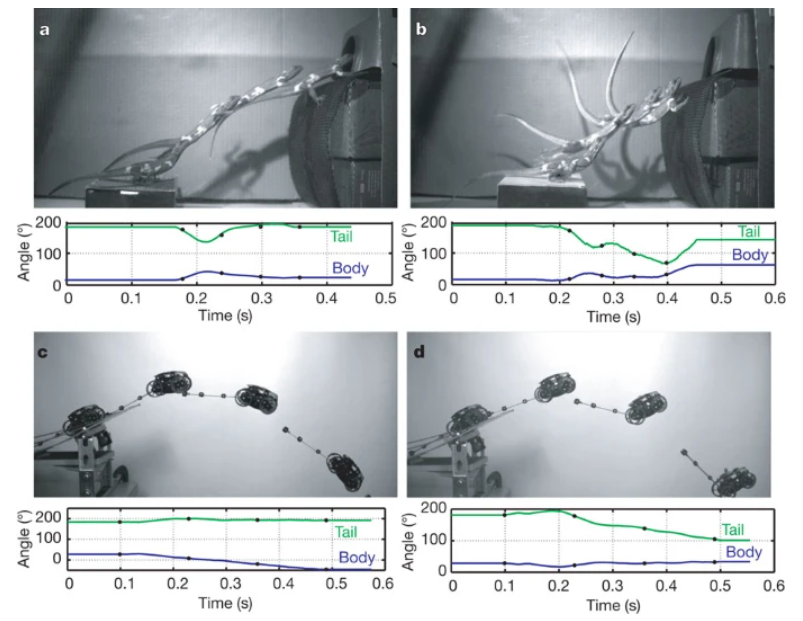
\includegraphics[scale=0.6]{agamaJump}
\caption{An Agama lizard compared to the Agama robot whilst jumping \citep{agama}.}
\end{figure}

\subsubsection{Leg Movement}
\label{sec:Leg Movement}
The approach to the fundamental movement of the legs is inspired by the Salamandra Robotica II \citepmain{salamandra}. Rotating each leg $360^\circ$ in its joint is a simpler mechanism to push the body forward than a biological folding limb. Though the design is somewhat detached from a biological leg, it is hoped that the implementation of a gait will restore a lizardlike motion.\\
To replicate a lizard's gait, diagonally opposite legs will be accelerated in rhythm with the motion of the body. 
\begin{figure}[H]
\centering
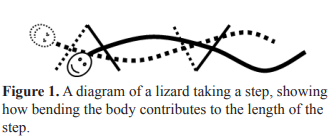
\includegraphics[scale=1]{lizardGait}
\caption{A representation of the relationship between a lizard's gait and its body oscillation \citep{reptileLocomotion}.}
\end{figure}
\nocitemain{reptileLocomotion}

\newpage
\subsubsection{Genetic Algorithm}
\label{sec:Genetic Algorithm Aims}
Evolution can be used as a \textit{"method for designing innovative solutions to complex problems"} \citepmain[p. 4]{gaIntro}. Lizardbot aims to emulate the biological evolution of lizards to find the optimal solutions among the many thousands of possible robot permutations: a mimicry of natural selection.
Thus, a genetic algorithm (GA) was chosen as an appropriate AI approach due to their \textit{"abstraction of biological evolution"} \citepmain[p. 1]{gaProsCons}. As Xin-She Yang discusses, GAs are suited to Lizardbot's broader optimisation problem, as they are fit for independent agents operating parallel to each other and for complex problem spaces \citepmain{gaProsCons}. Additionally, Lizardbot is not searching for a global optimum - in which case a \textit{"GA will have a good chance of being competitive with or surpassing other "weak" methods"} \citepmain[p. 116]{gaIntro}. However, the parameter values used by the GA can undermine its success: \textit{"inappropriate choice will make it difficult for the algorithm to converge or it will simply produce meaningless results"} \citepmain[p. 2]{gaProsCons}. \\
Overall, due to the properties of the problem space, a GA was considered to be the best option.\\

Genetic algorithms are formed of three main processes: selection, mutation, and recombination (or crossover) \citepmain{gaIntro}. The first of these is used slightly differently by Lizardbot. Conventionally, all agents would be considered each generation and a select few recombined/mutated. Instead, an algorithm will determine when a robot is stuck and terminate the generation of that robot in isolation - evolving the population asynchronously. \\

The mutation stage randomly adjusts a selection of the genes to allow for random variations to form in the population. Mutation can \textit{"[insure]
the population against permanent fixation at any particular locus"} \citepmain[p. 129]{gaIntro}. Essentially, mutation avoids convergence within the population and encourages the formation of new solutions. 

The recombination stage mimics the genetic crossover that occurs when two animals produce offspring. The 'breeding' will occur between the selected robot and another chosen either for its physical or movement similarity. Alternatively, a \textit{Triad} method breeds all three of these together. The offspring of three successful robots is expected to be more successful than the conventional two. A parallel in nature is the multiple matings found in Harvester ants, improving colony performance via \textit{"increased genetic variance within the worker population of the colony"} \citepmain[p. 1601]{antMating}. It goes without saying that even with multiple matings there will still be the traditional two genetic inputs. However, there is a connection between the two methods and their \textbf{opportunity} for genetic diversity. \\
The \textit{Triad} method also aims to strengthen the relationship between body and movement. As discussed in \ref{sec:Evolution Gym}, Evolution Gym's co-design GA mutated these two mechanisms in tandem and produced higher-performing robots in most tasks being tested \citepmain{evolutionGym}.\\

Another option explored is a \textit{Lizard} method whereby the mate is selected proximally using a characteristic with no direct impact on performance. Male spiny-footed lizards appear to favour redder females - a trait that appears to signal sexual maturity \citepmain{redLizard}. For these lizards the body colour appears to signal sexual maturity, a physiological trait that can impact on the success of the population but is not as direct a causation as traits usually considered to be desirable (e.g. signs of health, fighting ability) \citepmain{lizardWeapon}.\\
For this project, the desirable trait is the body colouration; Lizardbot loves blue. In theory, this method should create local ‘ecosystems’ in the population over time as robots that explore the same area of the terrain each iteration will always interact with the same selection pool. \\

The genetic algorithm aims to optimise the parameters of Lizardbot and, once an optimal robot has been found, could be removed from the project. It has no impact on the behaviour of the robot mid-generation in reaction to specific circumstances.\\

\newpage
\subsubsection{Dynamic Movement}
\label{sec:DST Aims}
\begin{wrapfigure}{r}{0.3\textwidth}
    \centering
    \vspace*{-5mm}
    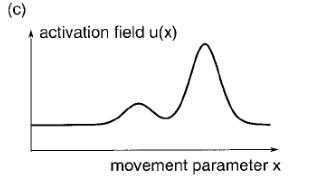
\includegraphics[width=0.3\textwidth]{activationExample}
    \caption{An example of a movement being activated: weakly at first, then again with a stronger activation to produce a greater movement \citep{dft}.}
    \label{fig:activationDiagram}
\end{wrapfigure}
\nocitemain{dft}
Dynamic systems theory uses the causal webs of an environment to determine the \textit{"sequences of states that could take the system from one location in state space to another"} \citepmain[p. 122]{mindware}.\\
Rather than providing rigid rules about how the robot should move, the robot explores how to move in a direction through trial and error. Essentially, it will 'collect' behaviours. If a specific set of parameters produced a desired behaviour (e.g. move left) then this can be activated with increasing force (see \autoref{fig:activationDiagram}) to steer the robot left across the terrain. This approach would produce a behaviour-based approach to navigating the terrain. Thelan and Smith explored the behaviour of babies taking steps on a treadmill and concluded that there was a complex relationship between the body, environment and behaviour \citepmain{babyStepping}. This relationship can be argued as both advantageous for Lizardbot, and a potential constraint to the performance that dynamic movement can offer.\\

The adaptive behaviour can result in emergent complex behaviours that would otherwise have been a mammoth of a task to implement as a set of instructions. On the flipside, dynamic movement relies on assumptions about the relationship between a robot's body, movement, and terrain. It is not feasible to store every factor that culminated in a behaviour and thus the system must be reduced to a select few control parameters. The assumptions that this requires render the dynamic approach unsuitable as the primary movement mechanism. However, it may still complement the movement algorithms discussed in \autoref{sec:Project Aims}. Andy Clark discusses the idea of "partial programs" \citepmain{partialPrograms} - \textit{"minimal instruction sets that maximally exploit the inherent (bodily and environmental) dynamics of a controlled system"} \citepmain[p. 133]{mindware}. As long as Lizardbot's adaptive behaviour can work alongside other causal influences then dynamic movement is expected to improve its performance.
 



\newpage
\subsubsection{Terrain Generation}
\label{sec:Terrain Generation}
Three terrains will be generated to test the robot in increasingly difficult environments. The terrains will be randomly generated once and then stored and used as a control variable in experiments.\\ 
The terrain types $[Smooth, Uneven, Rough]$ to be created are inspired by those used to test the Octopus robot \citepmain{octopusRobot}.\\

It is important to consider the situatedness of the Lizardbot. Herbert Simon provided an elegant example of the importance of this consideration: an ant is observed making its way back to its nest across a beach.
Its route is ‘a sequence of irregular, angular segments’ that suggests some level of complexity in the ant's behaviour. However, the beach for the ant is a much harsher environment than it is for a human. It is more likely that ‘its complexity is really a complexity in the surface of the beach, not a complexity in the ant’ \citepmain{antsBeach}. Thus, the situatedness of the robot could culminate in behaviours that are not of its own making and are instead caused by its relationship with the terrain. The smooth terrain should reduce the role of the environment and allow for emergent behaviours to be prescribed to the robot itself.\\

\subsection{Extension Objectives}
\label{sec:Extension Objectives}
\subsubsection{Vision}
\label{sec:Vision}
Thus far the Lizardbot has focused on finding the ideal parameters for the overall form and movement of the robot, with additional thought for a dynamic system to allow the robot to react to its situation. There has been little focus on a preemptive approach, which has the potential to reduce the risk of damage to a real robot. When a robot becomes stuck it will likely find itself bouncing against the nearby terrain, forcing the prioritisation of durability in the design of the robot. If the robot were given a rudimentary visual system it could instead anticipate collisions and adjust its course to avoid them.\\ David Lee investigated the factors affecting the specific moment in which an agent will begin reacting to an impending collision. He found that for an agent approaching a stationary object, the relative location of the obstacle in the agent’s visual field could be used to deduce the time-to-collision \citepmain{timeToCollision}. The use of this time-to-collision would directly relate to the brief of the project as it applies an algorithm derived from nature to a design problem (in this case collision detection and avoidance). \textit{”Most animals respond avoidantly and directionally to the abstract visual stimulus ... which specifies the approach of an object and impending collision”} \citepmain[p. 1]{animalCollisionResponse}.\\
Implementing a visual system to the Lizardbot could unlock a variety of more complex - \textbf{and proactive} - behaviours.

\newpage
\section{Project Relevance}
\label{sec:Project Relevance}
\subsection{Modular Snake Robot}
\label{sec:Modular Snake Robot}
The work of Ye et al. \citepmain{modularRobotBackground} found that a modular snake robot was \textit{“more efficient to get into complicated environments”} \citepmain[p. 453]{modularRobotBackground}. Their aim was to test the abilities of such a robot in environments too harsh for humans. Each module operated independently in a manner similar to the body movement algorithm covered in \ref{sec:Body Movement}. Each module was attached to the adjacent modules via a joint that rotated to create a wave through the body, whilst a servo drove the module forward. Their robot used a cosine function to manoeuvre the body, whereas Lizardbot will make use of an approach closer to that of a central pattern generator. \\
The modular snake robot successfully navigated any obstacles with a height less than the height of a module. It also demonstrated the constraints that a physical robot can face (e.g. the error rate in the servos increased with amplitudes over 4cm). Lizardbot aims to explore similar methods of movement to improve its environmental adaptivity, without the physical limits faced by the modular robot. The addition of legs and a tail to the modular design is intended to enable the robot to overcome more complex obstacles in its environment. Meanwhile the AI will, theoretically, allow the Lizardbot to adapt to its situation more than the modular snake robot was able to.

\subsection{Agama Robot}
\label{sec:Agama Robot}
The tail-assisted pitch control used to build the Agama lizard-inspired robot will heavily influence the tail motion of the Lizardbot \citepmain{agama}. It will constantly assess the momentum of the robot and adjust the motion of the tail to counterbalance this force. Applying this research may reduce the risk of the robot overbalancing, a situation that could damage a physical robot. The Agama study found that \textit{“the robot with PD feedback tail control maintained a nearly constant body angle by swinging its tail upward and incurred 72\% less rotation after a perturbation than did the robot without tail control”} \citepmain[p. 181]{agama}. This is a promising result for stabilising the Lizardbot.

\newpage
\subsection{Salamandra Robotica II}
\label{sec:Salamandra Roboticaa II}
The relevant goal of the Salamandra Robotica II \citepmain{salamandra} was to \textit{“advance robotics design for bimodal and efficient locomotion”} \citepmain[p. 309]{salamandra}. The design of this robot heavily inspired various elements of the design of the Lizardbot: the full rotation of the legs and the CPG-inspired oscillation of the body. \\
One of the key differences between the Salamandra and the Lizardbot is the method for turning. The former used calculated asymmetric oscillations to produce a curving trajectory (see \autoref{fig:salamandraTurning}) while the latter will dynamically derive an activation function for a turn. \\
\begin{figure}[H]
\centering
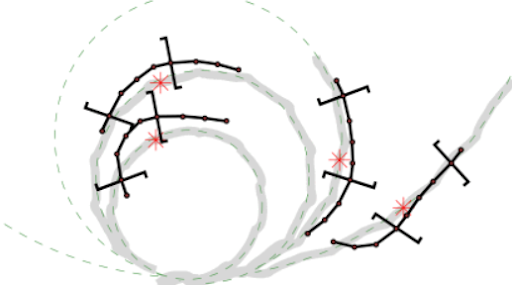
\includegraphics[scale=0.7]{salamandraTurning}
\caption{The results of various curved trajectories of the Salamandra \citep{salamandra}.}
\label{fig:salamandraTurning}
\end{figure}
Another difference was the Salamandra’s passive tail. The tail fin was only used to test its effect on speed whilst swimming; removing it decreased the speed by 63\%. The rigidity of the tail will be matched by this project but, as previously discussed, it will rotate to counterbalance the motion of the rest of the body.

\subsection{Evolution Gym}
\label{sec:Evolution Gym}
Evolution Gym \citepmain{evolutionGym}, unlike the previous works covered in this section, modelled their robots rather than build them. It shared a common goal with Lizardbot: optimise the movement and body together using a co-design algorithm. \\
Evolution Gym likewise employed a (much simpler) genetic algorithm. Evolution was conducted synchronously using the top $x\%$ of the population and did not feature recombination. Other optimisation algorithms were tested against the GA on a series of both locomotion and manipulation tasks and the evolved robots were compared to a hand-crafted selection. The former were able to find a balance between their structure and motion in a way that the hand-crafted robots could not. Interestingly, the autonomously generated robots resembled \textit{"existing natural creatures"}\citepmain[p. 1]{evolutionGym} - a result that it is hoped Lizardbot will achieve too.

\newpage
\section{Requirements Analysis}
\label{sec:Requirements Analysis}
It is difficult to predict what the specific applications of this project would be and what range of possible constraints they may have. Are elements of the physical design restricted? What kind of terrain is the robot going to be placed in? Are there other factors that need to be accounted for, e.g. gravity, bodies of water? This project is designed to be broad such that it can be adapted for a narrower use case. It lays the groundwork for research tailored to creating a robot for bomb disposal, planet exploration, or even a robot hoover that can handle stairs!
The features that a target system would include are outlined here, split into functional and non-functional elements.

\subsection{Functional Requirements}
\label{sec:Functional Requirements}
\subsubsection{Realistic Physics}
\label{sec:Realistic Physics}
To achieve a suitable performance function, the robot will need to interact realistically with the terrain around it. If it were to remain on a ledge in a precarious position that any physical robot would have immediately fallen off then this is not a realistic model. 
This need was a significant factor in the decision to use Unity, as opposed to other modelling software such as MSC Adams \citepmain{mscAdams}. It is expected that collisions and gravity will be accurately modelled, with credit to Unity.


\subsubsection{Transferable Design}
\label{sec:Transferable Design}
It would be beneficial for the target user if there were a direct correlation between the design of the model and the physical structure of a robot based on the model. Lizardbot has a vague shape but the underlying structure would be transferable to a blueprint for a robot. The model will deliberately use realistic constraints to avoid outcomes that cannot be replicated (e.g. the maximum degrees of freedom will be bound).

\subsubsection{Risk Reduction}
\label{sec:Risk Reduction}
Regardless of its purpose, any user will want their robot to avoid behaviour that risks damage. This function can be somewhat achieved by having the AI predict the upcoming terrain and proactively decide how it will navigate it. The AI will introduce a bias toward robots that minimise their collision force: by avoiding collisions and falls, the largest risks can be reduced. \\
Additionally, the model could approach this objective via the proactive decision-making that has been established as a possible extension to the AI.

\subsubsection{Effective AI}
\label{sec:Effective AI}
It is important that the AI is capable of evolving an input population to a higher performing one over time. The constraints placed on it may limit its success; nonetheless it should display an upward trend.\\ The AI should minimise bias towards certain physical structures or behaviours to allow for more freedom in the resultant robots. 

\subsubsection{Dynamic Movement}
\label{sec:Dynamic Movement Req}
It would be advantageous for the user if Lizardbot were able to 'learn' from prior behaviour and reactivate this to explore farther across terrains. Dynamic movement aims to address this requirement and is predicted to provide a drastic improvement on the performance of a population.

\subsubsection{Multiple Terrains}
\label{sec:Multiple Terrains}
The robots evolved by the AI should show a similar performance when placed into a new terrain, to demonstrate that their motion is optimised for a range of environments as opposed to simply the one they were trained in.

\subsection{Non-functional Requirements}
\label{sec:Non-functional Requirements}
\subsubsection{Physical Testing}
\label{sec:Physical Testing}
A model is excellent for testing theories but can overlook the 'real physics' that becomes apparent when building a physical robot. For example, the modular snake robot needed to ensure that the robot had \textit{“enough space for installing the joint driving mechanism and the circuit modules”} \citepmain[p. 450]{modularRobotBackground}. \\
Unfortunately, building a physical robot would require time and expensive resources. It will not be possible to test the model’s performance on an actual robot. This will hopefully be compensated for by having a realistic physics system and a model whose design is directly transferable to the blueprint for a robot.

\subsubsection{Customisable Input}
\label{sec:Customisable Input}
A target user may already have known constraints for the design of their physical robot and wish to see this represented in Lizardbot. Likewise, the ability to model a specific environment may be valuable for modelling the effectiveness of a robot in a terrain it is going to encounter.
The parameters used by the project will be contained to \textit{Config} files that can be adjusted with minimal programming knowledge. However, it will not be possible to accomodate every criterion so a user may still need to extend the project to their needs. 
The current expectation is that the user will require some knowledge of Unity to interact with the project. The addition of a UI may be desirable in future to lower the technological threshold. 



\newpage
\section{Implementation}
\label{sec:Implementation}
\subsection{Terrain}
\label{sec:Terrain Imp}
Three terrains were generated using Procedural Toolkit \citepsoft{proceduralToolkit} to test the performance of the robot across various environments: rough, uneven, and smooth. 
\begin{figure}[H]
\centering
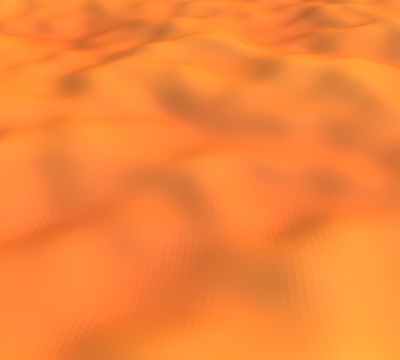
\includegraphics[scale=0.3]{smoothTerrain}
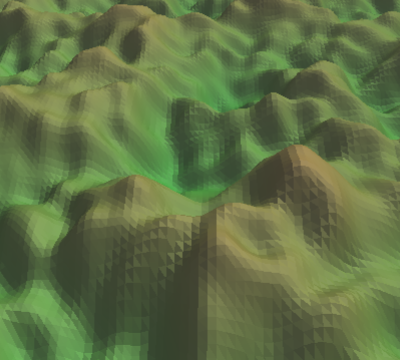
\includegraphics[scale=0.3]{unevenTerrain}
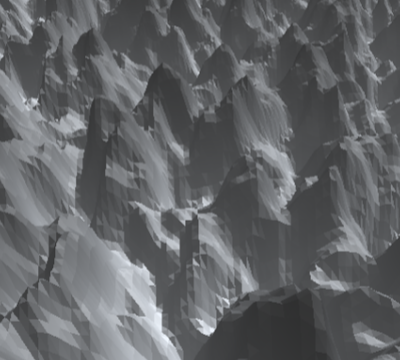
\includegraphics[scale=0.3]{roughTerrain}
\caption{Examples of the three terrain types. (From left to right) Smooth, Uneven, Rough.}
\end{figure}
At one point the height of the terrain was proportional to the number of sections of the robot, a similar method to that of the Octopus robot \citepmain{octopusRobot}. However, as the terrain is a control variable the heights were switched to a static value: $Smooth=8, Uneven=16, Rough=24$.\\
Overall, the rougher the terrain, the higher and more closed in it is. Most of the development of the robot was conducted on the smooth and uneven terrains, as the rough terrain aims to provide a more extreme environment with which to test the efficacy of the AI.\\
It is worth noting that the three terrains do share some common properties (e.g. gravity) and these factors may introduce bias in the AI. For proof of concept the sample set of terrains is sufficient.\\


\subsection{Robot}
\label{sec:Robot Imp}
\subsubsection{Body}
\label{sec:Body Imp}
To create a snakelike body, each body module is attached to the previous module by a configurable joint \citepcode{configJoints} and has two methods of movement: driving and rotation. The physical design of the robot creates a fluid motion before any complex movement is applied. With the joint structure, the driving of one section is translated to those behind it - similar to dragging a piece of string along the ground. This is shown in \autoref{fig:bodyOutput}a: the head rotates and, after a delay, creates the same angle in the sections behind it.\\

Meanwhile, the rotation applies a velocity to each of module using the following equation:
\begin{center}
\begin{Large}
$\overrightarrow{v_{i}} = \overrightarrow{v_{i-1}} + \frac{m}{2}\overrightarrow{w} $
\end{Large}
\end{center}

For rotating sections $i = 0, ..., m$, where $m \leq n$ (total number of modules), the value of $w$ will be calculated using $S$ or $C$ as specified.\\
\begin{center}
\begin{Large}
$S: \overrightarrow{w} = sin\overrightarrow{\theta_{i-1}} + sin\overrightarrow{\theta_{i}}$
\\[1\baselineskip]
$C: \overrightarrow{w} = cos\overrightarrow{\theta_{i-1}} + cos\overrightarrow{\theta_{i}}$\\
\end{Large}
\end{center}

This central pattern generator (CPG) inspired approach allows each module to react to the velocity and angle of the previous section. The equation for the CPG originated in Tony Dear’s multi-link snake robot: a robot with a similar modular design with passive joints connecting the modules \citepmain{cpgRobot}. Lizardbot utilises the same math to calculate the velocity with one distinction: Dear’s robot split the velocity vector into its axes, using cos for the x axis and sin for the y. Lizardbot instead calculates the vector as a whole and alternates the rotating sections between sin and cos to produce the serpentine motion. For robots with serpentine motion disabled, $S$ and $C$ will be assigned randomly to the $m$ rotating modules.\\

It is worth noting that every velocity calculated (for a body module, leg or tail) is multiplied by a parameter that can be mutated by the AI. Mostly it affects the primary axis of rotation, which allows the path of motion to be adapted over time.

\begin{figure}[H]
\centering
\centerline{
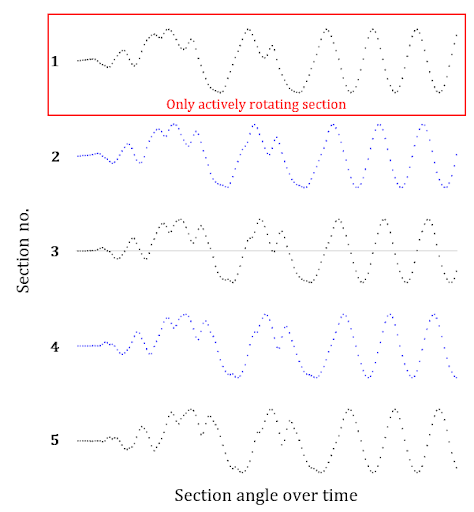
\includegraphics[width=0.6\textwidth]{cpgMirroring}
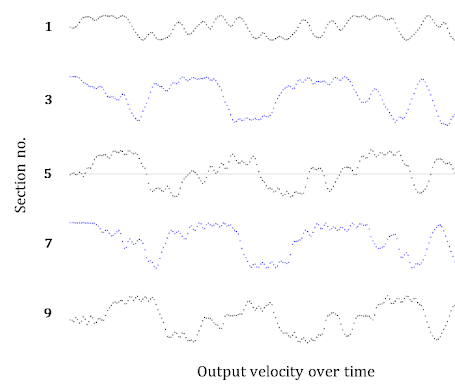
\includegraphics[width=0.6\textwidth]{cpgSerpentine}
}
\caption{(a) Left, (b) Right\\
(a) Demonstration of body motion with a single rotating section at the head of the body.\\
(b) The output velocities generated by each body module with serpentine motion enabled. Modules using $S$ are shown in black, $C$ in blue.\\
Created using Grapher \citep{grapher}.}
\label{fig:bodyOutput}
\end{figure}

For serpentine motion, each section ‘reacts’ to the previous one whilst using the opposing equation to output a velocity that is almost an inversion of its predecessor. Moving back through the body there appears to be more fluctuation in the values as more noise is introduced through each application of the equation. The advantage of using this recursive approach is the incredibly organic behaviour that it produces. The first prototypes of the project used hardcoded timings and velocities to try and mimic a serpentine motion and the rigidity of the code was evident in the behaviour. With the above equation applied, the motion of the body appears completely natural. As the Lizardbot slithers through troughs in the terrain or wriggles whilst stuck on a ridge, it is easy to forget that it has no awareness of its surroundings. It is simply reacting to the body that came before it.

\newpage
\subsubsection{Tail}
\label{sec:Tail Imp}
A tail has the potential to counterbalance the body and provide stability as the robot moves. The Agama robot used the angular momentum of the body to calculate how to calibrate the tail vertically as the robot jumped. Lizardbot implemented a similar approach in three dimensions by calculating the total momentum of the robot around its centre of gravity (COG) at each frame, and adjusting the velocity of the tail accordingly.\\ 
\begin{figure}[H]
\centering
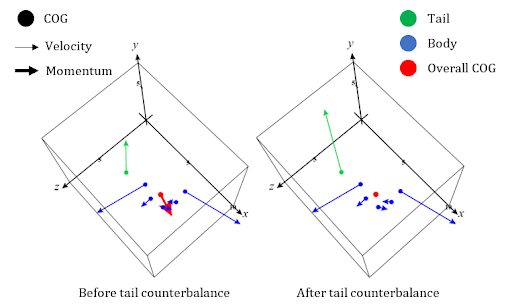
\includegraphics[scale=0.6]{tailMomentum}
\caption{A representation of the tail being adjusted to conserve the angular momentum of a robot. Diagram created using CalcPlot3D \citep{diagrams}}
\end{figure}

For all body parts $i = 0, ..., n$, the radius of the path of motion $r$ is the distance from the individual COG $x$ to the COG of the overall robot.
\begin{center}
\begin{Large}
$r = |x_{i} - \frac{1}{n}\sum_{i}^{n}m_{i}x_{i}|$
\end{Large}
\end{center}

The total angular momentum $L$ of the robot is calculated using the above values of $r$, the mass $m$ and the velocity $v$ of each body part \citepcode{angularMomentum}.
\begin{center}
\begin{Large}
$L = \sum^{n}_{i} r_{i}m_{i}v_{i}$
\end{Large}
\end{center}

To conserve momentum, the velocity of the tail is calculated by inverting $L$ and dividing it by the tail's mass and distance from the overall COG.
\begin{center}
\begin{Large}
$v_{t} = - \frac{L}{r_{t}m_{t}}$\\
\end{Large}
\end{center}

Another simplified approach was considered whereby the overall velocity of the robot was counterbalanced instead. However, this was found to create sharp changes in the velocity of the tail that could cause it to fling the entire body into the air. Whilst this showed promising behaviour for the basis of a jumping motion, it was counter-productive for a feature whose goal was to stabilise the robot. Additionally, by accounting for the COG, any difference in mass between components is taken into consideration. Thus, the tail is able to counterbalance any body structure (assuming that the motion of the tail is not physically blocked by the position of a body part).\\

The design of the tail assumes that nature has already selected for the optimal location by placing the tail at the back of a creature. This assumption seems intuitive: most animals, including lizards, are symmetrical. The location of the tail maintains this property whilst keeping the motion of the tail in the same plane as the rest of the body. In future, this assumption could be removed to explore how the position of the robot affects the robot. Who am I to say that a tail cannot be located on the head?

\subsubsection{Legs}
\label{sec:Legs Imp}
Legs were added to Lizardbot in an attempt to model the gait of a lizard.
As inspired by the design of the Salamandra Robotica \citepmain{salamandra}, each leg is designed to rotate in a circle to push the body forward. The physical design of the leg matches the elliptical shape of the tail and uses the same configuration of customisable mass and length. 
Currently, there are only two attachment points for a leg on each body module: one each side, perpendicular to the body joints. For a uniform body, the legs are placed symmetrically along the body and given equal length and mass; they are constructed randomly for non-uniform bodies. \\

The leg rotates around an axis perpendicular to the body section it is attached to, as shown in \autoref{fig:legRotating}. The size of the circle it follows is determined by the angle it is offset by when attached to the body ($\alpha$). \\

\begin{figure}[H]
\centering
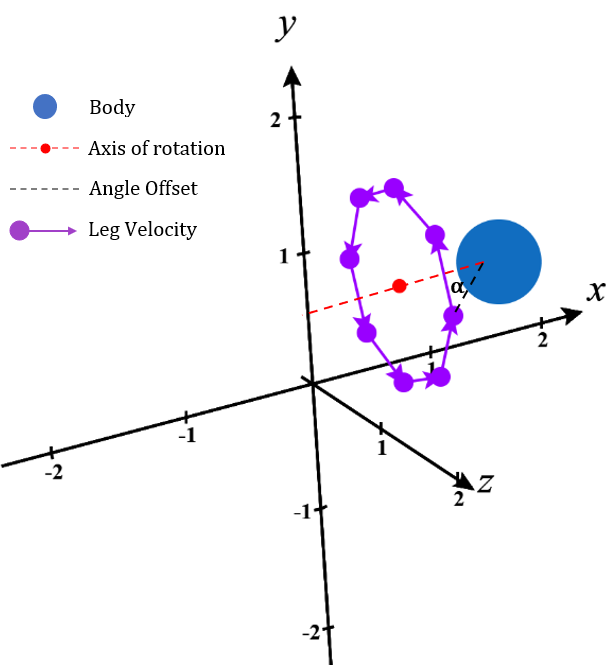
\includegraphics[width=0.5\textwidth]{legCircleDiagram}
\caption{An illustration of the rotation of a leg around an axis of rotation. Only one attachment point is shown - another would be available on the other side of the body along the $x$ axis. Diagram created using CalcPlot3D \citep{diagrams}.\\}
\label{fig:legRotating}
\end{figure}



The rotation of the leg follows a series of conceptual points spaced $30^\circ$ apart around centre point $D$ (shown by the red point on the axis of rotation in \autoref{fig:legRotating}). These points are generated using the following equation:
\begin{center}
\begin{Large}
$P = D + Vcos\theta + Ucos\theta$\\
\end{Large}
\end{center}

Where $V$ and $U$ are two vectors perpendicular to each other in a plane through $D$ and the target circle, and $0\leq\theta<360$ \citepcode{circlePoints}.
 
To calculate the desired velocity of the leg, the point $P_i$ closest to the current position of the leg is found. From this, the new velocity can be calculated using the vector to the next point on the circle.   
\begin{center}
\begin{Large}
$v_{i} = g(P_{i + 1} - P_{i})$
\end{Large}
\end{center}

If the relevant gene is active, the gait multiplier $g$ increases the velocity when the body is turning away from the leg, decreasing it if the body is turning toward the leg.\\

Currently the leg motion resembles a lot of twitching. It is possible that an alternative joint mechanism would allow for Lizardbot to stand on its legs and appear more natural. It would also be interesting to explore how the location of the legs impacts the robot as a whole. Currently the attachment points are based on lizards (indeed, most animals) and the years of evolution that have led to their structure. However, the offer of more variety in the design of the robot may offer alternative solutions to navigate the terrain. 


\subsection{Artifical Intelligence}
\label{sec:AI Imp}
A population of Lizardbots uses a genetic algorithm to "evolve" over a series of generations. A genetic algorithm is a form of artificial intelligence that more closely models the characteristics of natural selection. An agent’s parameters are broken down into ‘genes’ that can be manipulated by recombination and/or mutation. The aim of this genetic algorithm (GA) is to improve the performance of the robots over time. The GA is performed when a robot is declared to be stuck by the trapped algorithm. 

\subsubsection{Performance}
\label{sec:Performance Imp}
The metric used to measure the performance of a robot can heavily influence the outcome of the genetic algorithm. As the desired outcome is a robot capable of navigating the terrain, the base measurement used is the furthest distance (by magnitude) that it has travelled in a given generation from its spawn point within the terrain. 
\\[1\baselineskip]
Two additional parameters are used to add context to this base measurement. 

The first rewards robots that move quickly. The current performance is multiplied by the average speed (distance / time) of the robot since it spawned.

The second penalises robots that cause large collisions. Every time a body part encounters a collision it triggers a method that will measure the force that the body part has experienced. Unity's built-in physics system returns the impulse $I$ of a collision. Using this, the force can be found by dividing the impulse by time: {\Large $f = \frac{I}{t}$} \citepcode{collisionForce}.
If the force is found to be above a threshold then the robot will be penalised by deducting 10\% from the performance. 

This ensures that the robot is not evolving toward a behaviour that carries it across the terrain efficiently but would cause damage to itself in the physical world. An example of this is an iteration whereby the robots were observed ‘flicking’ their tails rapidly downward, causing the robot to be thrown into the air and across the terrain. Whilst this was effective at getting them to the edge of the terrain within seconds, this approach would shatter most robots. This threshold can be tailored to the needs of the robot, such that robots with shielding or soft bodies can be given a higher threshold to allow more risky behaviour.\\

A flaw in this metric is that it does not differentiate between the routes that robots take. If one robot moved quickly but erratically, it may be rewarded equally to one that moved slowly and directly. However, this metric appears to provide a suitable balance between rewarding robots that travel the farthest, further rewarding those that move efficiently, and reducing behaviours that would damage a physical robot. \\

When referring to the performance of a population, the mean performance of the top 25\% is being measured. It was found that analysing the entire population added too much noise to the results, as when a robot is mutated and respawned its performance returns to zero.

\newpage
\subsubsection{Trapped Algorithm}
\label{sec:Trapped Imp}
It is important for the AI to know when the robot is stuck to terminate its current generation. This trapped behaviour can take many forms: from bouncing against the same point in the terrain to circling itself.\\

The locations of the robot over the last $t$ seconds are analysed. The algorithm finds the minimum and maximum values for each axis to draw a conceptual cube around the points the robot has visited in the last $t$ seconds. These cubes depict the  worldspace the robot has recently explored. The variance of the data set is calculated for the volume of the cube rather than the coordinates themselves. If the variance of the volumes of the cubes converges to zero then the robot is considered to be trapped. \\
\begin{figure}[H]
\centering
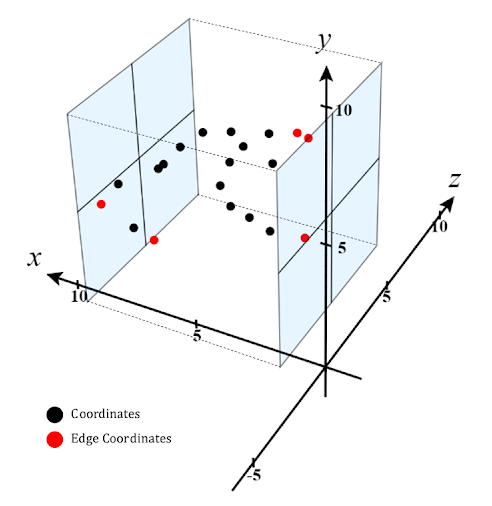
\includegraphics[scale=0.5]{trappedAlgorithm}
\caption{A representation of the cube constructed around the last 20 locations a robot has visited (captured twice a second). Diagram created using CalcPlot3D \citep{diagrams}.}
\end{figure}

The red points in \autoref{fig:trappedPoints} align with behaviours that can reasonably be classed as ‘trapped’, however it is important to note that this algorithm was implemented with some bias toward certain behaviours (e.g. looping). For this project, the identification of a trapped robot appears sufficient and is expected to produce an AI that will train away from continually exploring the same area for too long. The algorithm has other potential applications in finding looping patterns in any problem that can be assigned a worldspace. For example, a neural network could be analysed with this algorithm to determine when it is ‘stuck’ whilst performing a task, or a search algorithm could implement it to avoid excessively exploring within a section of the graph. 

\begin{figure}[H]
\centering
\centerline{
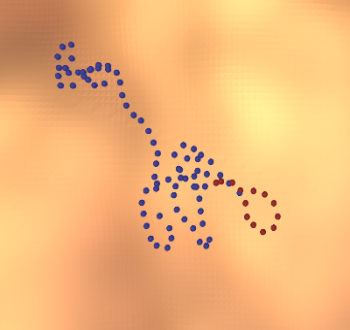
\includegraphics[width=0.25\textwidth]{trappedSmooth}
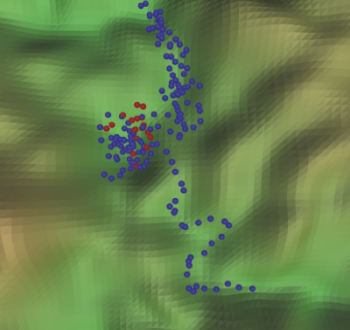
\includegraphics[width=0.25\textwidth]{trappedUneven}
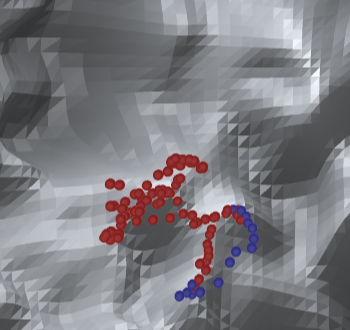
\includegraphics[width=0.25\textwidth]{trappedRough}
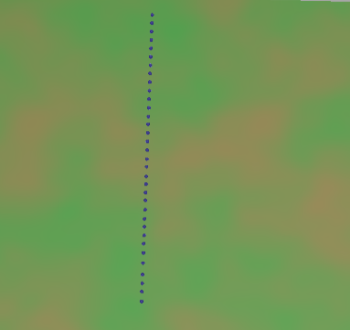
\includegraphics[width=0.25\textwidth]{trappedFlat}
}
\caption{A demonstration of the trapped algorithm using the same robot and $t=20$ on each terrain.\\
Each blue point represents the location of the robot being captured. Red indicates that the robot is trapped (and would normally have been disabled and passed to the genetic algorithm).\\ 
(From left to right) Smooth, Uneven, Rough, Flat. The latter used a robot with rotation disabled to ensure that a robot travelling in a straight line would not be flagged.}
\label{fig:trappedPoints}
\end{figure}


\subsubsection{Genes}
\label{sec:Genes Imp}
The manipulatable characteristics of a robot are distinguished by a \textit{Gene} class. Each variable is instantiated with a default, minimum, and maximum value. Additionally, they are given a type (established in the enum class \textit{Variable} whereby negative enum values are physical properties and positive are movement). \\
This class handles any erroneous situations that arise and allows boolean values to be stored as a float. If the \textit{Get} method of a boolean \textit{Gene} is called, then true will be returned for values greater than 0.5. This allows boolean genes to be mutated slowly (e.g. from 0.35 to 0.6) without having to make a single jump from one value to the other. \\

\subsubsection{Genetic Algorithm}
\label{sec:GA Imp}
When the trapped algorithm determines that a robot is stuck it is disabled and passed to the genetic algorithm (GA).\\

The mutation cycle of a robot refers to how many evolutions should take place before the resultant robot is compared to the robot it initially branched from. When a mutation cycle is complete, the highest performing of the two is selected as the input for the GA. The reasoning behind this is to allow a robot to mutate to a lower performing robot temporarily, as this may allow it to evolve into a more successful robot a few generations later.\\

Once the input robot has been determined, this robot is then recombined. There are several methods of recombination available but the overall process is: select $k$ robots using a given method and "breed" the genes of one robot in this pool with those of the input robot.\\
The available recombination methods are:
\begin{enumerate}
  \item Physical\\
The selection pool consists of robots that are physically similar to the input robot. The acceptable margin of difference is increased until k robots are found. This method aims to evolve the input robot toward another that is built similarly and is outperforming its current design.
  \item Movement\\
The selection pool consists of robots that are moving in a similar way to that of the input robot. As above, the acceptable margin of difference is incrementally widened if necessary. This method ignores the structure of the robot and instead evolves it towards another that is following the same movement rules but more effectively.
	\item Triad\\
This approach is more artificial than others. Two robots are selected: one each from the physical and movement methods. The genes of these two robots are then recombined with the input robot. As discussed in \ref{sec:Genetic Algorithm Aims}, nature does demonstrate examples of more than two agents mating. Lizardbot here explores how multiple mating partners might be beneficial when (unlike nature) all contributers are able to input their genetics.
	\item Lizard\\
This method aims to mimic a more lizardlike breeding process. Those with bluer body colours are selected, ignoring those in the population on the other side of the terrain. \textit{Nearby} is relative to the spawn point of the robot, and limited to those in the same terrain type. 
	\item Performance\\
In line with more conventional GAs, the highest performing $k$ robots are collected and a random robot within this pool is selected for recombination. Methods 1-3 aim to evolve the input robot toward a more successful version of its current form. This method instead disregards its current design and looks at the entire population instead.
	\item Random\\
A random robot is selected from the population, to act as a control method.
	\item Any\\
Methods 1-5 make an assumption that using the same method for every generation is optimal. This method instead randomly selects one of the above methods for a single generation.
\end{enumerate}
Each of the input robot's $n$ genes is recombined as follows:
\begin{center}
\begin{Large}
$G(1)_{i} = R^{[0, 1]} < r \longrightarrow$ 
\begin{LARGE}
$^{R^{[0, 1]} < 0.5\longrightarrow G(1)_{i}} 
_{R^{[0, 1]} \geq 0.5 \longrightarrow G(2)_{i}}$
\end{LARGE}
\end{Large}
\end{center}

Where $i = 0, ..., n$. R denotes a randomly generated number in the range $[a, b]$. G(1) refers to the input robot, whilst G(2) is the selected robot. For \textit{Triad} recombination G(2) is randomly chosen from either of the two selected robots, with equal probability.\\

The recombined robot is then mutated. The genes are divided into physical or movement properties to allow the mutation to be limited to one or the other, or both.
The mutation rate $m$ is used to avoid mutating every single gene.\\
When a gene is mutated its value is adjusted as follows:
\begin{center}
\begin{Large}
$G_{i} = R^{[0, 1]} < m \longrightarrow $
$(max(G_{i}) - min(G_{i})) R^{[0.01, 0.1]}  G_{i}$\\[1\baselineskip]
\end{Large}
\end{center}
The mutation could be improved by switching from an adjustment of $1-10\%$ of the gene range, to instead using Gaussian noise \citepmain{gaussian}.\\

The GA contains four major parameters that influence its function: recombination rate, mutation rate, selection size, and mutation cycle. To determine the optimal values for these, 47 iterations were run with randomly generated values and the performance of the population measured. Each iteration contained 50 robots running for 600 seconds.
The desired outcome was a performance curve that sloped upwards over time. Peaks and troughs were expected as the successful robots returned to the spawn point; the overall pattern of the performance was key. 
\begin{figure}[H]
\centering
\centerline{
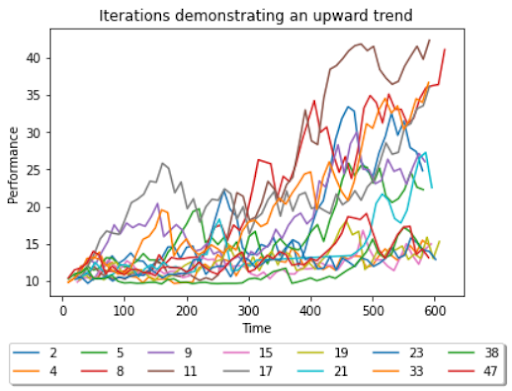
\includegraphics[width=0.6\textwidth]{gaPatternIterations}
\includegraphics[width=0.6\textwidth]{gafilteredIterations}
}
\caption{(Left) All iterations demonstrating a promising upward trend.\\
(Right) Iterations from the left graph filtered to those that reached a performance $>20$.\\
Graphs created using Colab \citep{colab}, Pandas \citep{pd}, MatPlotLib \citep{plt}, and NumPy \citep{np}.}
\end{figure}

Upon analysing the four values being used for the highest performing upward-trending iterations it appeared that successful values had been found through an issue in the code. When generating random values, Unity cycles through the same values if not provided with a seed \citepcode{randomRepeating}. As the four values were consistently the first four values generated they had been repeatedly set as $[2, 0.77, 0.31, 9]$. Of the 8 iterations that showed an upwards trend and performed well, 7 were these values. Additionally, there was only a single iteration using these values that did not perform well. Given the apparent success of these GA values, these were selected as the default parameters. \\
It would be useful to have different GA parameter values tailored to each combination of the recombination and mutation methods. Currently, effective values have been found whilst the \textit{Any} option was selected for both in an attempt to find parameters suitable for all permutations. However, this may favour certain combinations more than others and there is currently no data on this. Rather, these base values are assumed to be appropriate and the effectiveness of the methods themselves judged relative to them. \\

\subsection{Dynamic Movement}
\label{sec:DST Imp}
As outlined in \ref{sec:DST Aims}, a dynamic approach uses the historical movement of the robot to ‘learn’ how to move in a given direction again. 
Take a robot that moves left by rolling over. Due to the reactive nature of the algorithms used for movement, it can be assumed that applying the same velocities from the start of the roll would produce another leftward motion. The dynamic movement algorithm saves these velocities for use when a robot needs to move left again. \\
\begin{wrapfigure}[14]{r}{0.3\textwidth}
    \centering
    \vspace*{-5mm}
    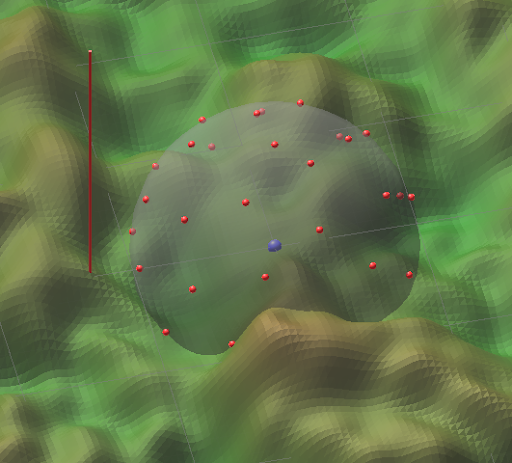
\includegraphics[width=0.3\textwidth]{spherePoints}
    \vspace*{-7mm}
    \caption{A sphere created using a Fibonacci lattice ($n=50$) around a centre point shown in blue.}
\end{wrapfigure}
To achieve this, the worldspace around a robot is divided. \textit{“The Fibonacci lattice is a simple way to very evenly distribute points [on the] surface of a sphere”} \citepmain[sec. 0]{fibonacci}. Using the implementation of the Fibonacci sphere provided by Fnord \citepcode{spherePoints}, a series of $n$ points were constructed in a sphere around the robot. It was necessary to strike a balance between too low a value of $n$ producing inaccurate results, which could cause the robot to veer off to one side of the intended direction. Meanwhile, too high a value of $n$ would be unnecessarily expensive and result in the majority of the points containing $null$ values. $n=50$ was selected as an appropriate granularity.\\

The sphere points are relative to the centre of the sphere, thus acting as vectors in the direction of the point. To track how the robot moves in a direction, every $t$ seconds the velocities of each body part are stored. A conceptual sphere is constructed around the initial position of the robot and adjusted to match its rotation. This way, a point directly to the left of the robot rotated $30^\circ$ around an axis will be in the same relative location to the robot at $120^\circ$. \\
Given another interval of $t$, a vector is calculated from the initial position to the resultant position. The sphere point closest to this vector is found by comparing the angle between the vector and the points. 
If there are already values stored for this point then the set of values that moved the robot the furthest distance in the time interval are saved. This process of saving the velocities used to move toward a point is illustrated in \autoref{fig:storeVelocities}. 
\begin{figure}[H]
\begin{minipage}[t]{0.3\textwidth}
\centering
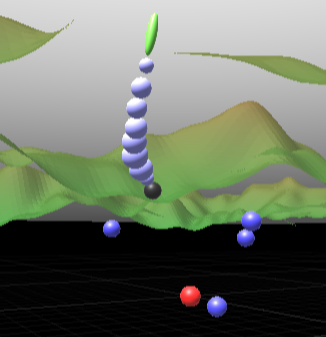
\includegraphics[width=1\textwidth]{storingVelocities}
\vspace*{-7mm}
\caption{Each blue point represents a set of stored velocities for a robot that moved left before turning right and moving downward.}
\label{fig:storeVelocities}
\end{minipage}
\hfill
\begin{minipage}[t]{0.65\textwidth}
\centering
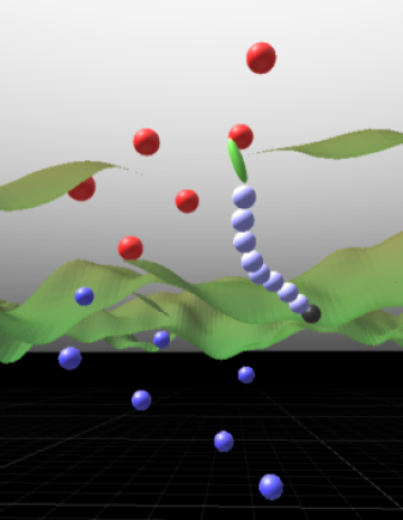
\includegraphics[width=0.4\textwidth]{dstFiltered}
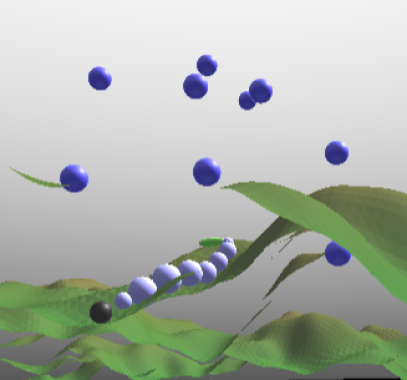
\includegraphics[width=0.55\textwidth]{dstFilteredMissing}
\vspace*{-3mm}
\caption{(Left) A wedge of points that would take the robot away from its spawn point. Those shown in red are those remaining after filtering for the height of the terrain.\\
(Right) An example of the terrain height filtering missing a point.} 
\end{minipage}
\end{figure}

\noindent There are two situations in which the motion of the robot is adjusted:
\begin{enumerate}
\item Routine adjustment\\
The goal of this adjustment is to keep the robot moving away from its spawn point. Every $x$ seconds the vector between the spawn point and the current position of the robot is calculated. The sphere around the robot is filtered using this vector to output a vertical wedge of points moving away from the origin. Applying any of the velocities saved at these points would theoretically direct the robot further across the terrain. \\
The points are further filtered by removing those that have not had any velocities stored yet and those that would move the robot below the level of the terrain. Due to the varying height of the terrain, three measurements are taken at incremental distances from the robot. If the direction of the point at this distance would take it below the height then it is removed from the selection. This method aims to take a snapshot of the rough height in a given direction and is liable to miss points that should be eliminated if the peak is between the snapshots. \\
From the filtered points, a single one is selected and the velocities applied to the robot. \\
Frequent adjustment may affect the ability of the robots to explore new means of movement. To reduce this, the regular adjustment is only enacted if the robot is not already moving toward any of the points in the initial wedge. 
\item Scaled adjustment\\
This adjustment is used when the robot is found to be stuck by the trapped algorithm.\\
At this point it is worth mentioning how the activation of the velocities is implemented. For the routine adjustment the applied velocities will be multiplied by a static activation rate. When a robot is trapped, this activation function is increased exponentially in an attempt to free the robot. Failing that, it is mutated and respawned. 
\begin{figure}[H]
\centering
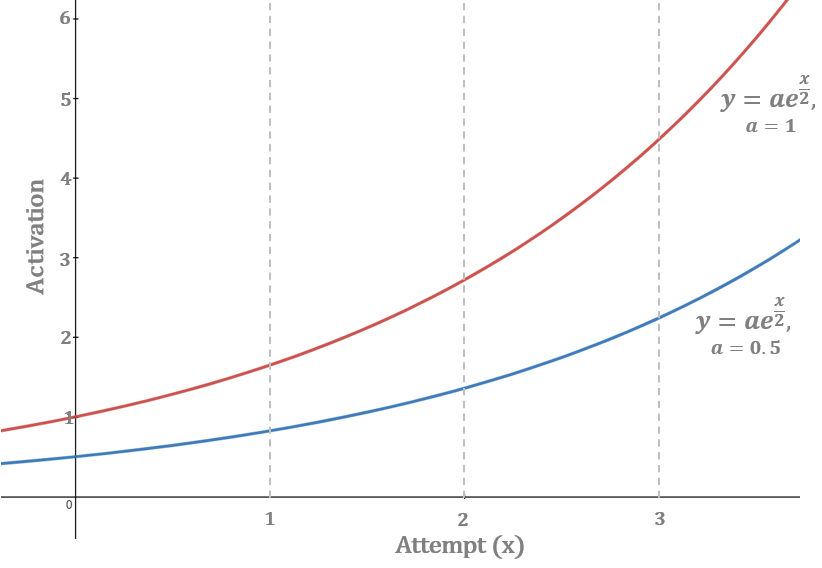
\includegraphics[scale=0.6]{activationFunction}
\caption{The activation multiplier used for each attempt at scaled adjustment. The static activation rate is shown as $\alpha$. Graph created using Desmos \citep{graphs}.}
\end{figure}
\end{enumerate}

It is expected that the dynamic movement algorithm will favour robots that are already performing well. All stored velocities are cleared when the robot is mutated, thus the robots will begin “learning” from scratch every time they become trapped. For robots with sufficient data about their movement, the scaled activation will theoretically enable them to progress in the terrain more often, thus reducing the mutation frequency. As they spend longer in the terrain, less successful robots will have longer to recombine with them. It is predicted that the dynamic movement will both improve the performance of any individual robot, and increase the rate of improvement across a population. \\

\newpage
\section{Results}
\label{sec:Results}
For each experiment discussed in this section the population was capped at 50 robots. This is an unfortunate constraint of the project due to technical limitations. My laptop had begun making some concerning noises and the university lab computers were incompatible with the project. As such, the data is a snapshot of what Lizardbot may be capable of at a larger scale.\\

All graphs are made using Colab \citep{colab}, Pandas \citep{pd}, MatPlotLib \citep{plt}, and NumPy \citep{np}.

\subsection{Body Motion}
\label{sec:Body Res}
\begin{wrapfigure}[17]{r}{0.5\textwidth}
    \centering
    \vspace*{-5mm}
    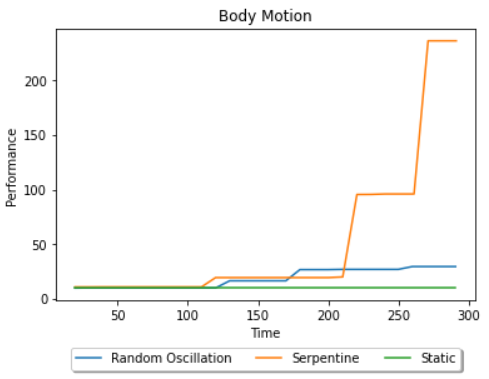
\includegraphics[width=0.5\textwidth]{bodyResults}
    \vspace*{-7mm}
    \caption{The results of different methods of body motion.}
    \label{fig:bodyRes}
\end{wrapfigure}
To test the effectiveness of the body motion, a population of 50 robots with 10 modules (no legs or tail) were measured with three forms of motion. All experiments measuring the efficacy of body parts were conducted on smooth terrain to avoid the situatedness of the robot impacting the results.\\
Random oscillation set random modules to rotate. Due to the embodiment of the robots this motion still resembled a coiling snake. This method outperformed a static body (driving only) which appeared to curve the body around the contours of the terrain. At the slightest gradient this caused the robot to become stuck. \\
As \autoref{fig:bodyRes} shows, the serpentine motion showed $\sim$5x the success of the random oscillation. Thus, serpentine motion became the default motion used in future experiments. 

\subsection{Counterbalancing Tail}
\label{sec:Tail Res}
\begin{wrapfigure}[16]{l}{0.5\textwidth}
    \centering
    \vspace*{-5mm}
    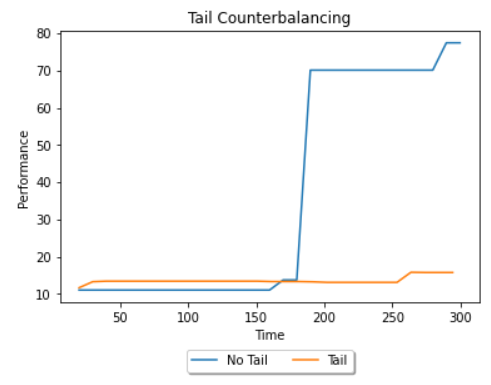
\includegraphics[width=0.5\textwidth]{tailResults}
    \vspace*{-7mm}
    \caption{The impact of tail counterbalancing.}
\end{wrapfigure}
The impact of a counterbalancing tail was analysed by comparing the performance of a tail-less serpentine body against one with a medium-length tail. The results were damning: the tail significantly limited the population. There are several theories behind this.

The first is that the physical parameters of the test tail were unsuitable. It would be useful to repeat this experiment with varying tail lengths and masses to determine if there is a tail form that complements the body. 

The second is that a rigid tail may be a less effective design. The tail could be observed colliding with the terrain at times which could have thrown the robot off its path of motion. The Agama robot tested a flexible robot and found that after a perturbation a rigid tail produced 72\% less impact; a flexible tail resulted in 85\% less rotation \citepmain{agama}. Given the performance of a serpentine body, applying this to a modular counterbalancing tail may render success. 

\newpage
\subsection{Leg Gait}
\label{sec:Leg Res}
\begin{wrapfigure}[17]{r}{0.5\textwidth}
    \centering
    \vspace*{-5mm}
    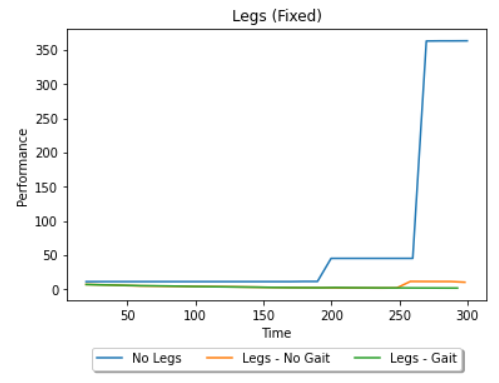
\includegraphics[width=0.5\textwidth]{legResults}
    \vspace*{-7mm}
    \caption{The impact of the addition of legs with/without a lizardlike gait.}
\end{wrapfigure}
To test the function of the legs, a serpentine 10-module tail-less body was compared against another with 6 legs positioned symmetrically. The latter robot was tested with and without the use of a gait. The results determined that both populations with legs performed terribly. This was not so surprising: as explained previously, the implementation of the legs has some room for improvement.

Interestingly, the use of a gait flatlined the performance. Given a more effective foundation for the legs, it may be that the gait concept would have worked. The Salamandra used a phase rotation between the body and legs to form a gait \citepmain{salamandra}. This more coordinated approach may have been more suitable than the simple increase in velocity in reaction to the motion of the body. \\

\subsection{Uniform vs Non-uniform Robot}
\label{sec:Uniform Res}
\begin{wrapfigure}[14]{l}{0.5\textwidth}
    \centering
    \vspace*{-5mm}
    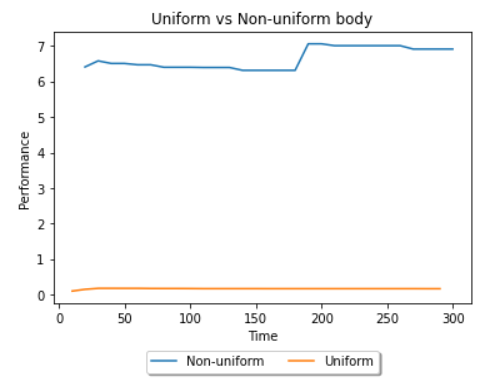
\includegraphics[width=0.5\textwidth]{uniformResults}
    \vspace*{-7mm}
    \caption{The results of a uniform vs non-uniform body.}
    \label{fig:uniformRes}
\end{wrapfigure}
A population of 50 non-uniform robots were created and left to execute for 300s. At this point they were toggled to become uniform, respawned and measured again. \\
The results, shown in \autoref{fig:uniformRes}, suggest that forcing a uniform body hindered the robots. There was next-to-no progress made by the uniform version of the robots after 300s. \\
The ability to force a uniform body was retained in the AI but, given the performance shown here, it is unlikely that this robot would remain in the population for long.
\\[2\baselineskip]

\subsection{Mutation Constraints}
\label{sec:Mutation Res}
\begin{wrapfigure}[12]{r}{0.5\textwidth}
    \centering
    \vspace*{-5mm}
    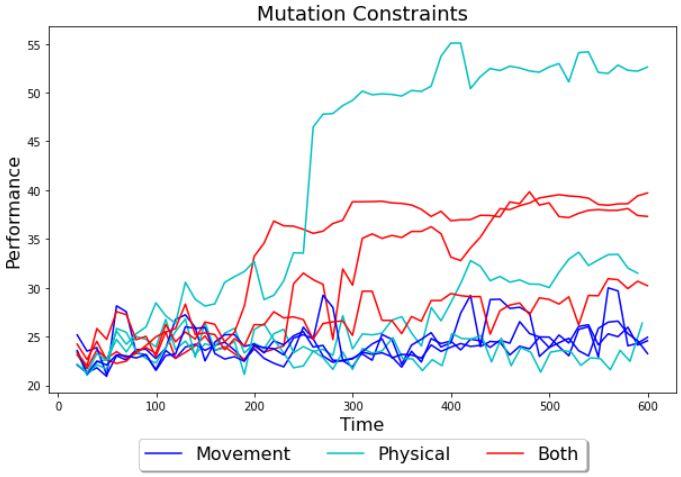
\includegraphics[width=0.5\textwidth]{mutationTypes}
    \vspace*{-7mm}
    \caption{The results of the GA constrained to physical/movement genes.}
\end{wrapfigure}
As explained in \ref{sec:Genetic Algorithm Aims}, there is the option to restrict the GA to only movement or physical genes. There are 18 permutations available between the mutation constraints and the recombination methods. Providing data for each would have been time-consuming and strained an already struggling laptop. Instead, the most effective constraint (using \textit{Any} recombination) was found and used for \ref{sec:Recombination Res}.
This was found to be the manipulation of all genes, which produced consistently high results.

\subsection{Recombination Methods}
\label{sec:Recombination Res}
\begin{wrapfigure}[18]{l}{0.5\textwidth}
    \centering
    \vspace*{-5mm}
    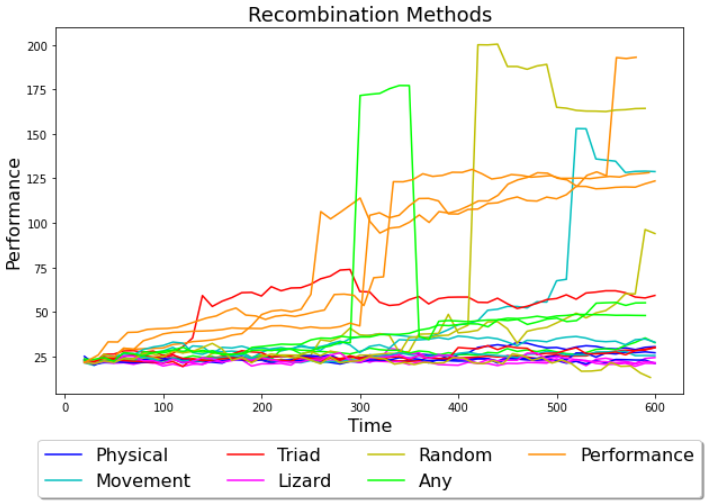
\includegraphics[width=0.5\textwidth]{recombinationTypes}
    \vspace*{-7mm}
    \caption{The results of each recombination method.\\ An outlier was excluded for a \textit{Random} iteration; a single value was recorded at 531.8821}
    \label{fig:recombinationRes}
\end{wrapfigure}
The \textit{Physical, Movement, Triad} and \textit{Lizard} recombination methods all produced disappointing results. \textit{Triad} achieved a single sucessful iteration, but was rejected as a viable option given the lack of progress elsewhere. One explanation for the demise of these recombinations is that the selection methods created localised breeding groups within the population. It may be that with active incest prevention \citepmain{gaIntro} these recombination methods would show more promise.\\
\textit{Any} recombination demonstrated a consistent (if slow) upward trend but still appeared less successful that the \textit{Random} control group.\\
The GA demonstrated consistently high performance with \textit{Performance} recombination. \autoref{fig:recombinationRes} shows the clear success of the top 25\% of the population. Beyond this, it was observed that almost every robot was consistently reaching the edge of the uneven terrain. However, there are still some fundamental issues with it.\\
A major issue is that not all genes have equal weight. If the gene that determines whether a uniform body is maintained mutates from false to true then this has a significant effect on the robot. The physical properties of almost all body and leg parts will be adjusted, resulting in a much larger adjustment to the robot than those caused by mutating other genes. Similar large-scale adjustments are applicable when moving to serpentine motion.\\
To mitigate this, it would be useful to apply weights to each gene. Thus, the mutation range could be scaled accordingly, or the genes categorised such that a change to a heavily weighted gene would limit any changes to other genes. This would allow an isolated analysis of the effect that such a large mutation has on the performance.\\

There is an assumption within the GA that asynchronous evolution is superior to synchronous evolution. The alternative would be to allow every robot to operate for $x$ seconds before mutating a percentage of the population in parallel. This would ensure that every robot experiences the same number of generations and remove any assumptions in the algorithm used to declare a robot as trapped. \\
Intuitively, the current approach is more appropriate as it does not leave unsuccessful robots continuing past the point where they have been identified as trapped. It is also more natural: we do not wait for a person’s 30th birthday before allowing them to have children based on how successful they have been thus far in their lives. \\

\newpage
\subsection{Dynamic Movement}
\label{sec:DST Res}
The addition of dynamic movement had an interesting impact on the performance graph. Seemingly, it results in a high-performing solution significantly better than those without. The exception to this (first graph in \autoref{fig:dstRes}) is suspected to be due to the GA (with dynamic movement) not having enough time to finish converging. Dynamic movement comes at a cost: it creates a delay in finding a solution and converges to a single solution with no further improvement.
\begin{figure}[H]
\centering
\centerline{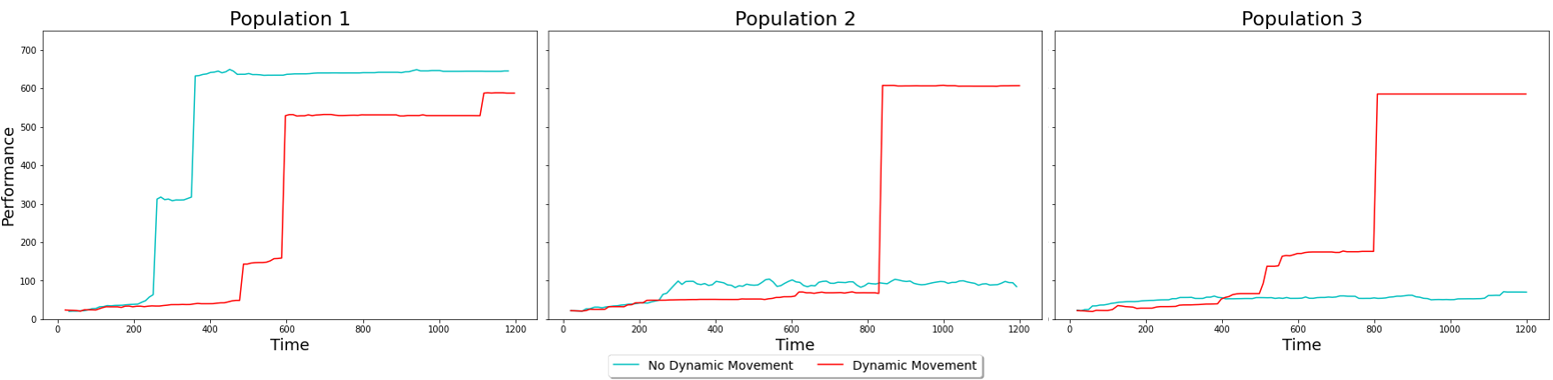
\includegraphics[scale=0.55]{dstResults} }
\caption{The impact of dynamic movement on three separate randomly generated populations. Uneven terrain was used, and a GA with \textit{Performance} recombination and no mutation constraints.}
\label{fig:dstRes}
\end{figure}
The dynamic movement could be further improved by performing a more comprehensive analysis of the entire terrain around the robot and making a more informed decision about the direction the robot should move in. This could further prevent the robot from becoming trapped as it avoids higher ground, or alternatively uses a larger activation to “jump” onto it.\\

\subsection{Evolved Robots}
\label{sec:Robot Res}
The final experiment that was conducted explored how the GA and dynamic movement performed across each of the three terrains. Much of the testing had been focussed on the smooth and uneven terrains so the use of the rough terrain would provide insight into the overall success of Lizardbot. Unsurprisingly, the performance on the two easier terrains was exemplary: one iteration on the uneven surface reached a performance of 15946.23!  This result was replicated and is not considered an outlier.

However, progress was slow on the rough terrain. This suggests that Lizardbot in its current form is limited to moderate environments rather than the harsher ones it was targeting. \\

It is possible that Lizardbot could be improved by repeating the honing of the GA parameters on the rough terrain. It was presumed that calibrating it on the uneven terrain would produce a scaleable GA; this assumption may have introduced bias towards easier environments.  
\begin{figure}[H]
\centering
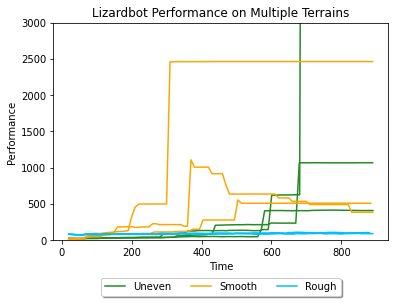
\includegraphics[scale=0.8]{multipleTerrains}
\caption{The outcome of the GA (with dynamic movement) across each of the three terrains. The uneven graph that is not fully visible continues to $15946.23$ and remains within range of that value.}
\end{figure}

Where the results get interesting is in the form of the final evolved robots. The first two terrains evolved the entire population to a single module that drove with speed between the troughs. There was no intention of producing these results but the fumbling balls were undoubtedly an optimal solution. These sped across the terrain - even 'climbing' over peaks - and consistently hit the edge of the terrain within seconds. This speed is likely the reason behind the 16k performance shown by the uneven terrain. \\
There was a slight differentiation between the resultant robots from the smooth and uneven terrains. The latter produced heads of similar size to each other. Contrastingly, the former gave rise to robots that were both smaller and varied in size. Though a single module has been found as an optimal design, there are still variations within this structure that can tailor it to its environment. \\
The GA on the rough terrain deviated from this rolling ball result, instead constructing a short string of modules, a tail, and symmetrical legs for 2/3 robots. It is worth taking these resultant robots with a pinch of salt due to their performance.\\

\begin{figure}[H]
\centering
\centerline{
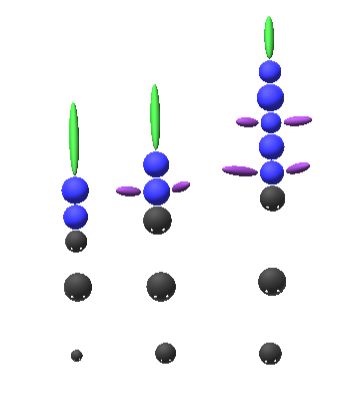
\includegraphics[width=0.2\textwidth]{best-above}
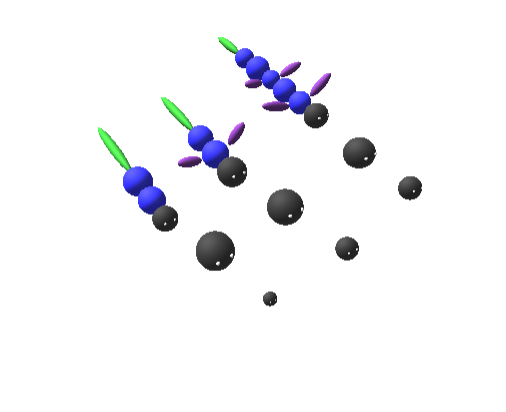
\includegraphics[width=0.35\textwidth]{best-side}
}
\caption{The highest performing robots evolved by the GA. The rows correspond to each terrain: rough, uneven and smooth respectively (from top to bottom).}
\end{figure}

\newpage
A behavioural analysis was conducted by placing these 9 robots back onto each terrain (with the GA disabled). As expected, all 6 balls immediately began rolling across the smooth terrain. On uneven, only the larger ones were able to traverse the environment whilst the smaller ones (evolved on the smooth terrain) became stuck in a trough. Thus far, the bodied robots had remained still. 

On the rough terrain the rolling behaviour became unproductive. All six balls immediately rolled into a basin and remained there. For the others, it appeared that the tail helped the robots 'push' themselves up steep slopes and the twitching legs provided sudden boosts in velocity. It is possible that more productive legs would have greatly improved the performance here by pushing them further than the (very) short distance they achieved.

\newpage
\section{Conclusion}
\label{sec:Conclusion}

The goal of this project was to produce a nature-inspired model of a robot that could navigate rough terrain. The majority of the inspiration was reptilian, supported by research indicating the efficient and adaptable motion of snakes and lizards. The modular body, counterbalancing tail and lizardlike gait had already been proven to be effective by works such as the Agama robot and Salamandra Robotica. \\

The results of Lizardbot corroborated the efficacy of serpentine motion. However, the data suggested that the movement of the tail and legs were counterproductive to the success of the robots. Seemingly, the snakelike design had been implemented more effectively than the lizard-inspired design aspects.\\ 

A genetic algorithm was used to mimic a biological evolutionary process. The GA was found to be limited regarding which terrains it could find a suitable solution for. The goal was optimisation for navigating rough terrain; the outcome was a GA that can optimise for moderate terrain. However, the reasons behind this could be overcome given more time. The parameters used were targeted at the uneven terrain - which produced phenomenal results - and as such a GA tailored to the harsher environment may yield a higher performance. Ideally, a single GA would work across any terrain.\\
Lizardbot could further be improved by exploring the option of a flexible tail (see \ref{sec:Tail Res}) or by applying the algorithm to a larger population to reduce the formation of localised breeding groups. Additionally, the introduction of a visual system (see \ref{sec:Vision}) could provide proactive collision avoidance to complement the collision penalisation in the performance metric. \\

Dynamic movement encouraged the robots to manouevre away from their spawn point. This feature was proved to improve the performance of the population at the cost of a convergence on a single solution. Whilst effective, this may have restricted Lizardbot from finding more abstract solutions. \\

The evolution of the robots produced unexpected results that deviated from the natural evolution of lizards. The optimal solution was found to be a single ball rolling with speed across the terrain. Whilst the basis of the project was to produce a nature-inspired solution, an effort was deliberately made to not enforce or bias towards a naturalistic robot. Evolution does not always offer an efficient or elegant solution; the laryngeal nerve in giraffes is a prime example of this unintelligent design. This nerve connects the brain to the larynx in most mammals but diverts under the heart instead of taking the direct path through the head and neck. In giraffes this results in a highly inefficient 5m laryngeal nerve \citepmain{giraffeNerve}. Arguably, the emergence of such non-natural robots suggests the successful avoidance of bias in Lizardbot. Perhaps in thousands of years lizards too will have evolved into a rolling sphere. 

\newpage

\section{References}
\label{sec:References}
\nocitesoft{*}
\nocitecode{*}

\bibliographymain{References/References}
\bibliographysoft{References/SoftReferences}
\bibliographycode{References/CodeReferences}
\newpage


\section{Appendices}
\subsection{Progress Logs}
The status of Lizardbot was reported as the project progressed.
The progress logs for Lizardbot can be found here:\\
\url{https://github.com/jacobgeorge26/lizardbot/pull/10}\\

\noindent The details of the discussions with the project supervisor, Simon Bowes, can be found here:\\
\url{https://github.com/jacobgeorge26/lizardbot/pull/9}


\subsection{Project Proposal}
The initial project proposal can be found here:\\
\url{https://docs.google.com/document/d/17SvBZN9ctZutAxGG5i6fcNnbd7-2hrrye14ARTxWUa4/edit?usp=sharing}



\end{document}